\section{Discussion}

Our study provides the first direct empirical test of the long-standing hypothesis that wind disrupts overwintering monarch butterfly clusters. For over three decades, conservation practice has operated under the assumption that wind speeds exceeding 2 m/s force butterflies to abandon their roosts, either by physically dislodging them or triggering behavioral departures \parencite{leongEvaluatingManagementCalifornia2016}. Our findings challenge this fundamental assumption and suggest a more complex relationship between monarchs and their overwintering environment.

\subsection{Evidence Against Wind Disruption}

The evidence against the wind disruption hypothesis emerges from multiple, independent lines of analysis. Most strikingly, every single observation period in our day-to-day analysis experienced maximum wind speeds exceeding the proposed 2 m/s threshold (range: 2.0--12.8 m/s), yet monarch clusters persisted throughout the 78-day study period. If the hypothesis were correct, we should have observed either mass departures when temperatures permitted flight or butterflies physically dislodged and littering the ground when too cold to fly, as described in the literature \parencite{leongRestorationOverwinteringGrove1999}. We observed neither.

Our bivariate analyses provide additional refutation. When we examined the simple relationship between wind speed and cluster size changes, we found essentially no correlation at either temporal scale (30-minute: r = 0.04, n = 1,894; day-to-day: r = 0.13, n = 96). These analyses tested the most basic prediction of the hypothesis: that increasing wind speed should produce decreasing cluster sizes. The absence of this relationship across wind speeds ranging from calm condidtions to six times the proposed threshold suggests that wind alone does not drive clustering decisions.

Statistical power was not a limitation. Our analysis achieved 87.5\% power to detect moderate effects and 98.5\% power for large effects. The wind disruption hypothesis predicts substantial, observable impacts, not subtle statistical signals. Our failure to detect these effects, despite adequate power and validated methodology that successfully identified other environmental signals, provides strong evidence against the hypothesis rather than merely absence of evidence.

\subsection{A More Complex Environmental Response}

While wind alone showed no disruptive effect, our models revealed that monarchs respond to environmental conditions through complex interactions, particularly between wind and solar exposure. This interaction emerged as the dominant environmental signal in both temporal analyses (30-minute: F = 4.67, p < 0.001; day-to-day: F = 4.10, p < 0.001), suggesting that the relationship between wind and monarch behavior depends critically on light conditions.

When butterflies experienced no direct sunlight, wind speed had no discernible effect on cluster dynamics across the entire observed range (0--12.4 m/s). However, when butterflies were exposed to direct sun, the combined effects of wind and light produced unexpected patterns. At intermediate levels of both wind and sun exposure, cluster sizes increased rather than decreased. This counterintuitive finding suggests that wind's role may be fundamentally different from what has been assumed.

One possible interpretation is that wind provides thermoregulatory benefits under certain conditions. \textcite{mastersMonarchButterflyDanaus1988} demonstrated that monarchs can dissipate heat while gliding, using airflow across their bodies for cooling. Environmental wind might provide similar cooling without the energetic cost of flight. When butterflies are exposed to direct sunlight, which can rapidly elevate body temperatures above optimal levels, moderate wind could help maintain thermal balance, allowing butterflies to remain clustered rather than dispersing to avoid overheating.

This interpretation remains speculative, but it aligns with the broader pattern of thermoregulatory responses we observed. Throughout our study, the strongest and most consistent environmental signals related to thermal conditions. Butterflies showed clear responses to direct sunlight, ambient temperature, and diurnal patterns, all of which influence body temperature. The wind-light interaction may represent another facet of this thermoregulatory challenge.

\subsection{Thermoregulation as the Primary Driver}

Beyond the wind-light interaction, our results consistently point to thermoregulation as the dominant factor shaping monarch clustering behavior. Direct sunlight alone showed strong effects independent of wind, with exposed butterflies showing the largest decreases in cluster abundance. This finding aligns with established physiology: monarchs in direct sunlight can elevate their body temperature above ambient conditions within minutes \parencite{mastersMonarchButterflyDanaus1988}. While this rapid warming enables flight at cool ambient temperatures, it becomes problematic when clustering, forcing butterflies to choose between the energetic benefits of aggregation and the risk of overheating.

Ambient temperature showed subtle effects within the range we observed (3.0--30.0°C), with patterns consistent with known thermal physiology. Minimal changes occurred below the 15°C flight threshold, while temperatures above 25°C triggered sharp declines in cluster size. These responses align with the fundamental challenge of overwintering: maintaining body temperatures cool enough to conserve energy through metabolic suppression, yet warm enough to permit essential movement \parencite{mastersMonarchButterflyDanaus1988}.

Time since sunrise revealed strong diurnal patterns (30-minute: F = 9.85, p < 0.001), with butterflies departing clusters in the morning and reforming aggregations in the afternoon. This pattern persisted even after controlling for temperature and sunlight, suggesting an endogenous rhythm that structures daily activity independent of immediate environmental conditions. Such predictable temporal patterns have been observed at overwintering sites throughout California \parencite{tuskesOverwinteringEcologyMonarch1978,chaplinEnergyReservesMetabolic1982}, indicating a fundamental aspect of overwintering behavior.

\subsection{Limitations and Context}

Several factors shape the interpretation of our findings. First, our data come from a single overwintering season (2023--2024) when monarch populations were relatively typical \parencite{xercessocietyWesternMonarchThanksgiving2025}. The following season saw near-complete absence of monarchs at our study sites, coinciding with the second-lowest overwintering population on record \parencite{xercessocietyWesternMonarchButterfly2025}. This dramatic population crash prevented temporal replication but underscores the urgency of understanding overwintering ecology with the data we have.

Second, our study observed relatively small clusters where butterflies maintained direct contact with eucalyptus substrates. The wind disruption hypothesis was developed during an era of massive aggregations containing hundreds of thousands of individuals, where many butterflies attached only to other butterflies in multi-layered formations \parencite{leongMicroenvironmentalFactorsAssociated1990,browerMonarchButterflyClusters2008}. If substrate attachment provides greater wind resistance than butterfly-to-butterfly attachment, wind might affect these different clustering configurations differently. The hypothesis may have been accurate for the extreme densities of past decades but less relevant to today's smaller populations.

Finally, our models explained relatively little variance overall (30-minute: 6.4\%; day-to-day: 39.7\%), reflecting both the complexity of butterfly behavior and our focus on testing specific hypotheses rather than comprehensively explaining movement patterns. However, the strong signals we did detect and our adequate statistical power give confidence in our main conclusion: wind alone does not disrupt monarch clusters as previously believed.

\subsection{Implications for Conservation}

Our findings suggest that strict adherence to wind protection thresholds may unnecessarily constrain habitat management. The absence of wind disruption despite frequent threshold exceedances indicates that suitable habitat within existing groves may be more extensive than currently recognized. Areas previously considered marginal due to wind exposure might support clusters if they provide appropriate thermal and light conditions.

However, we do not advocate abandoning tree planting or windbreak establishment. While wind protection may not directly prevent cluster disruption as previously thought, dense canopies provide other critical benefits: moderating temperature extremes, creating the dappled light patterns monarchs appear to prefer, and maintaining humidity levels that prevent desiccation. The fundamental practice of maintaining and restoring forest structure at overwintering sites remains sound, even if the mechanistic understanding requires updating.

Management focus might more productively shift toward understanding and maintaining thermal regimes within groves. As \textcite{sanieeHierarchyScaleInfluence2022} suggest, managing canopy structure to create appropriate light patterns and temperature gradients may be more important than achieving specific wind speed thresholds. This perspective aligns with our finding that the interaction between environmental factors, rather than single variables in isolation, shapes monarch clustering behavior.

\subsection{Future Research Directions}

Our findings open several important avenues for future research. The wind-light interaction we observed warrants direct investigation: does environmental wind actually provide thermoregulatory benefits to sun-exposed butterflies? Controlled experiments manipulating both wind speed and solar exposure while monitoring butterfly body temperatures could test this hypothesis directly.

The strong effect of light exposure also suggests that canopy structure may guide habitat selection more than previously recognized. \textcite{weissForestCanopyStructure1991} found that successful overwintering sites maintain consistent canopy openness around 20\%, while unsuccessful sites show greater variability (Figure~\ref{fig:weiss_canopy}). Combined with our findings, this suggests that predictable light patterns created by canopy structure may be a primary factor in roost site selection. Monarchs possess sophisticated visual systems that enable sun compass navigation during migration \parencite{nguyenSunCompassNeurons2021,mouritsenVirtualMigrationTethered2002}, capabilities that would allow them to detect and respond to consistent light patterns within groves.

\begin{figure}[h]
    \centering
    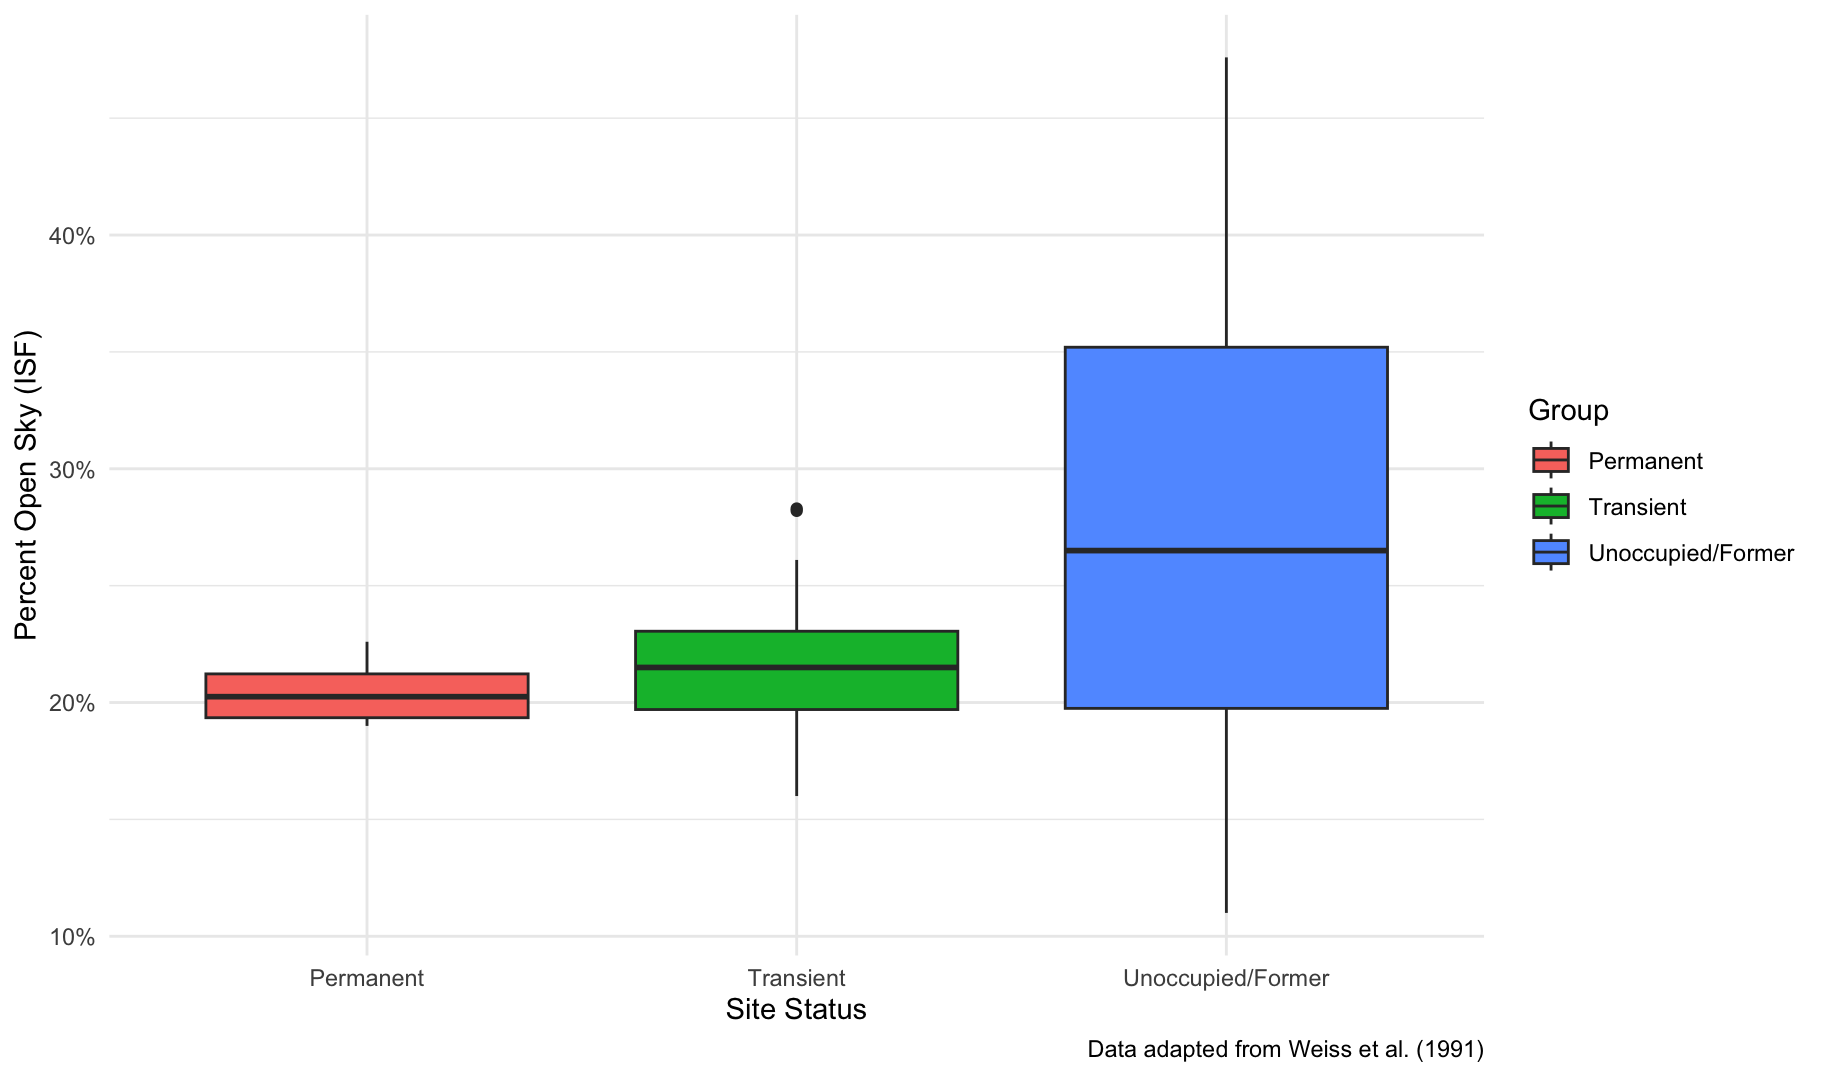
\includegraphics[width=0.8\textwidth]{figures/discussion/weiss_adapted_boxplot.png}
    \caption{Percent canopy openness (Indirect Site Factor) by occupancy status, adapted from Weiss et al. (1991). Permanent overwintering sites exhibit both a specific range of canopy openness (~20\%) and lower variance compared to transient and unoccupied/former sites.}
    \label{fig:weiss_canopy}
\end{figure}

Beyond environmental factors, social dynamics may explain additional variation in our models. The strong effect of previous butterfly count on subsequent changes suggests that monarchs do not distribute randomly within groves but rather exhibit overdispersed clustering patterns where the presence of butterflies attracts others. This positive feedback mechanism, where initial settlement increases the probability of others joining, could create self-reinforcing aggregation patterns independent of immediate environmental conditions \parencite{berdahlEmergentSensingComplex2013}.

Finally, testing these patterns across the broader overwintering range would establish their generality. Sites with different tree species, latitudes, and especially population densities could reveal whether wind responses vary with clustering configuration or if our findings represent fundamental aspects of monarch overwintering behavior.

\subsection{Conclusions}

Our direct test of the wind disruption hypothesis found no evidence that wind speeds above 2 m/s force monarchs to abandon their clusters. Every observation in our day-to-day analysis exceeded this threshold, yet clusters persisted. Bivariate analyses showed no relationship between wind and cluster changes. Model selection consistently identified other factors as more important. These multiple lines of evidence converge on a clear conclusion: wind alone does not disrupt overwintering monarch butterflies as has been assumed for over three decades.

Instead, our results point toward thermoregulation as the primary driver of clustering dynamics. Monarchs responded strongly to direct sunlight, ambient temperature, and diurnal patterns, all factors that influence body temperature. The unexpected wind-light interaction, where moderate wind combined with sun exposure sometimes increased cluster sizes, suggests that environmental conditions interact in complex ways that simple threshold-based management approaches cannot capture.

These findings arrive at a critical moment for monarch conservation. With western populations at historic lows, every assumption about habitat requirements deserves scrutiny. While our study cannot definitively explain why wind doesn't disrupt clusters or exactly how the wind-light interaction functions, it clearly demonstrates that current management guidelines rest on incomplete understanding. Moving forward, conservation efforts might more productively focus on maintaining thermal diversity within groves rather than achieving specific wind protection thresholds. As we face the challenge of preserving overwintering habitat for a declining population, evidence-based understanding of monarch ecology becomes not just scientifically important, but essential for the species' survival.